\documentclass[12pt, a4paper, simple]{eskdtext}

\usepackage{hyperref}
\usepackage{_env/gpi_global.env}
\usepackage{_env/gpi_report.env}
\usepackage{_sty/gpi_lst}
\usepackage{_sty/gpi_toc}
\usepackage{_sty/gpi_t}
\usepackage{_sty/gpi_p}
\usepackage{_sty/gpi_u}

% Переменные
\def \gpiDocNum {3}
\def \gpiTopicRep {Планирование создания программных элементов (ПЭ) для
автоматизированной системы обработки информации (АСОИ)}

% Код
% \ESKDletter{О}{Л}{Р}
% \def \gpiDocTypeNum {81}
% \def \gpiDocVer {00}
% \def \gpiCode {\ESKDtheLetterI\ESKDtheLetterII\ESKDtheLetterIII.\gpiStudentGroupName\gpiStudentGroupNum.\gpiStudentCard-0\gpiDocNum~\gpiDocTypeNum~\gpiDocVer}

\def \gpiDocTopic {Отчёт лабораторной работы №\gpiDocNum}

% колонтитулы
\usepackage{fancybox, fancyhdr}
\fancypagestyle{plain}
{
    \renewcommand{\footrulewidth}{0pt}          % Толщина отделяющей полоски снизу
    \renewcommand{\headrulewidth}{0pt}          % Толщина отделяющей полоски сверху
    \fancyhead[C]{ }                            % Коллонтитул сверху
    \fancyfoot[C]{\hfill\hfillстр. \thepage}    % Коллонтитул снизу
}

% Графа 1 (наименование изделия/документа)
% \ESKDcolumnI {\ESKDfontII \gpiTopic \\ \gpiDocTopic}

% Графа 2 (обозначение документа)
% \ESKDsignature {\gpiCode}

% Графа 9 (наименование или различительный индекс предприятия) задает команда
% \ESKDcolumnIX {\gpiDepartment}

% Графа 11 (фамилии лиц, подписывающих документ) задают команды
% \ESKDcolumnXIfI {\gpiStudentSurname}
% \ESKDcolumnXIfII {\gpiTeacherSurname}
% \ESKDcolumnXIfV {\gpiTeacherSurname}

\begin{document}
    \begin{ESKDtitlePage}
    \ESKDstyle{empty}
    \begin{center}
        \gpiMinEduRep \\
        \gpiEduRep \\
        \gpiKafRep \\
    \end{center}

    \vfill

    \begin{center}
        Тема: <<\gpiTopicRep>>
    \end{center}

    \vfill

    \begin{center}
        \textbf{\gpiDocTopic} \\
        по дисциплине \gpiDisciplineRep \\
    \end{center}

    \vfill

    \begin{flushright}
        \begin{minipage}[t]{7cm}
            Выполнил:\\
            \PageTitleStudentInfo
            \PageTitleDateField
            \hspace{0pt}

            Проверил:\\
            \PageTitleTeacherInfo
            \PageTitleDateField
        \end{minipage}
    \end{flushright}

    \vfill

    \begin{center}
        \PageTitleCity~\ESKDtheYear
    \end{center}
\end{ESKDtitlePage}

    \ESKDstyle{empty}
    \thispagestyle{plain}
    \pagestyle{plain}

    \begin{center}
        \textbf{\gpiDocTopic}
    \end{center}

    % = = = = = = = =
    \paragraph{} \textbf{Тема}: <<\gpiTopicRep>>

    \paragraph{} \textbf{Цель}:
    Формирование знаний и умений по планированию процесса создания ПЭ АСОИ.

    \paragraph{} \textbf{Планирование создание ПЭ}

    \textbf{Разработка общей логической структуры ПС АСОИ}.
    В качестве основы для построения логическая структура ПС используется функциональная модель ОА (см. рис. Г.1, файл ИндТреб).
    Логическая структура включает сле­дующие компоненты (см. рис.3.1):

    \begin{enumerate}
        \item[1.] Функциональная модель ОА (П1 - П5), которая определяет схему взаимосвязей между отдель­ными приложениями.
        При планировании реализации целесообразно учитывать связи между отдельными приложениями.
        \item[2.] Системные и прикладные программ (П0), которые необходимо приобрести на начала создания приложений ПС.
        \item[3.] Приложение эксплуатационного персонала (П6), которое реализуется в первую очередь.
    \end{enumerate}

    Представленная на рис. 3.1 общая логическая структура ПС представляет основные программные элементы ПС и связи между ними. 

    \begin{figure}[ph!]
        \centering
        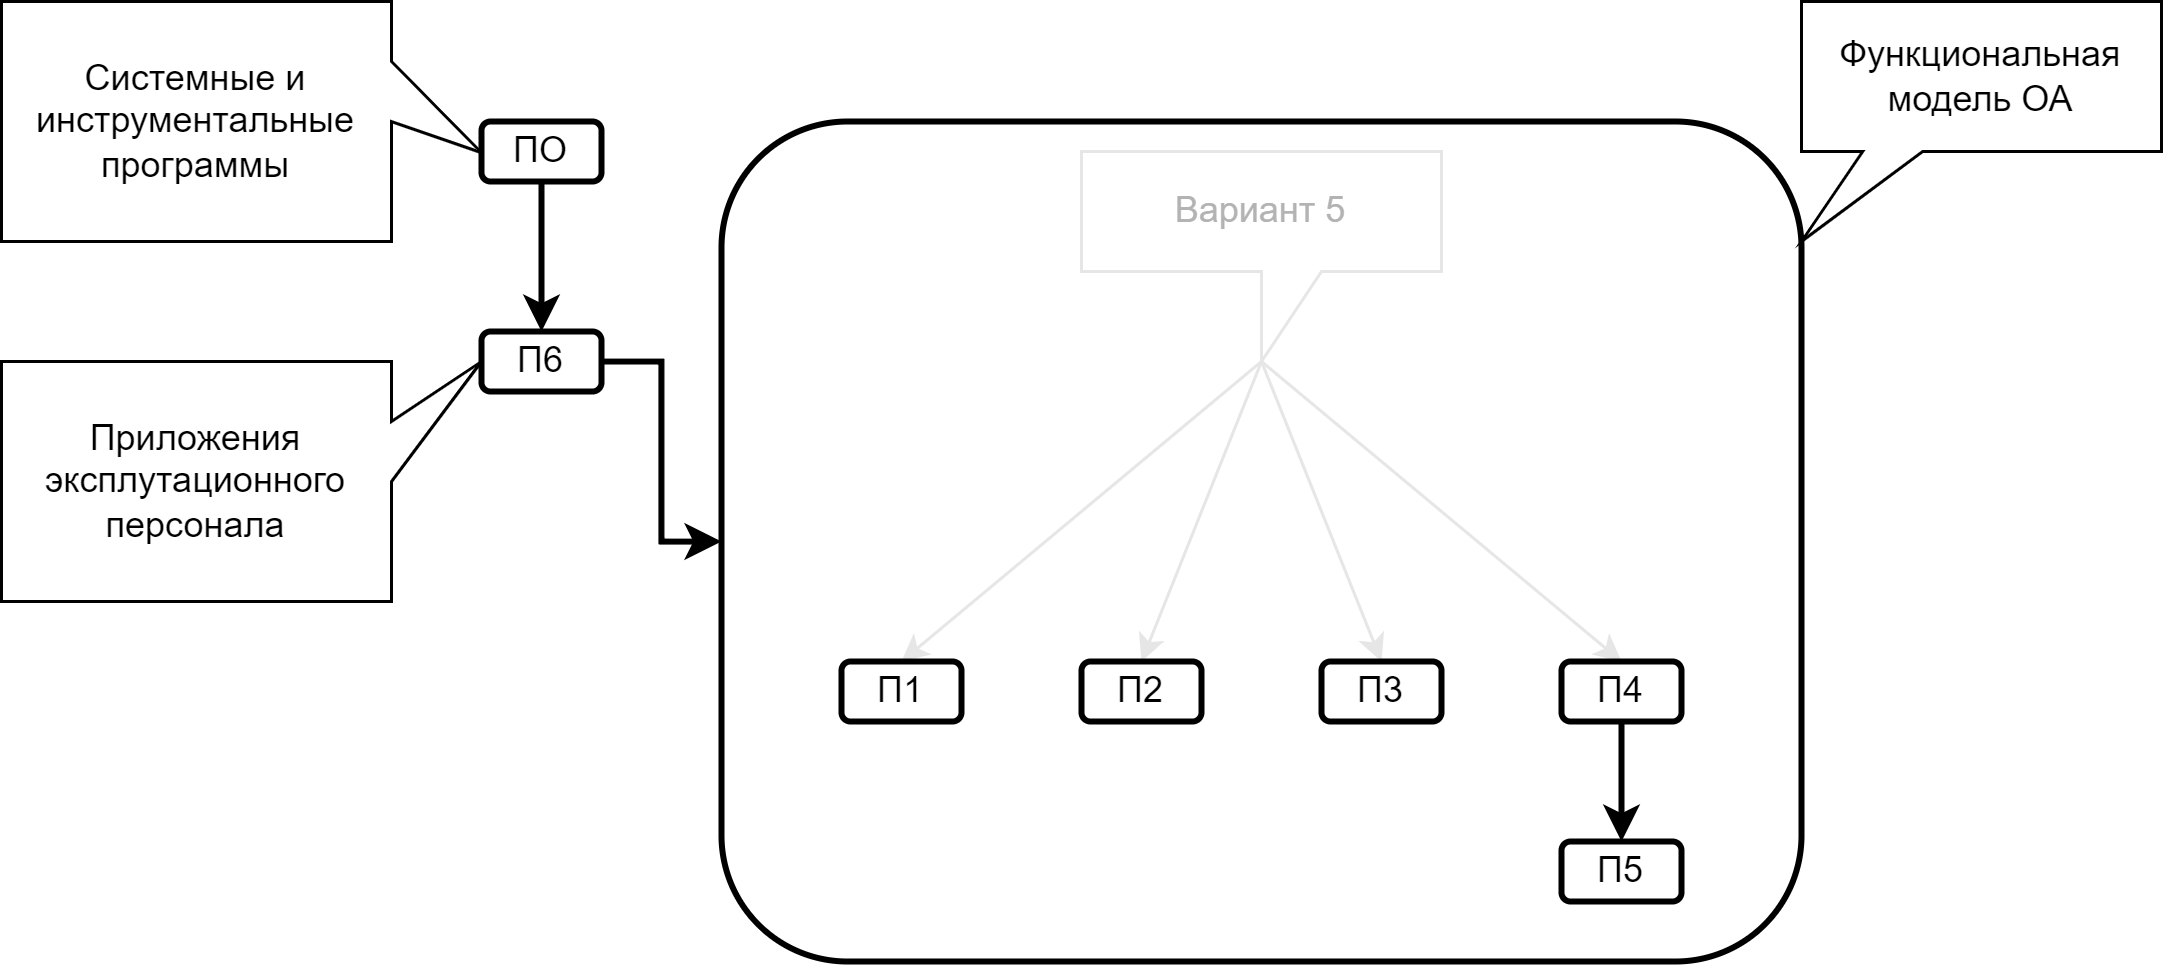
\includegraphics[width=16cm]
            {_docs/Рисунок3-1ПримерЛогическойСтруктурыПСАСОИ.png}
        \caption{Пример логической структуры ПС АСОИ}
    \end{figure}

    \newpage
    \textbf{Разработка сетевого процесса реализации ПС АСОИ}.
    Пример первоначального сетевого графика создания программ ПС приведен на рис. 3.2 для логической структуры ПС представленной на рис. 3.1. 

    \begin{figure}[h!]
        \centering
        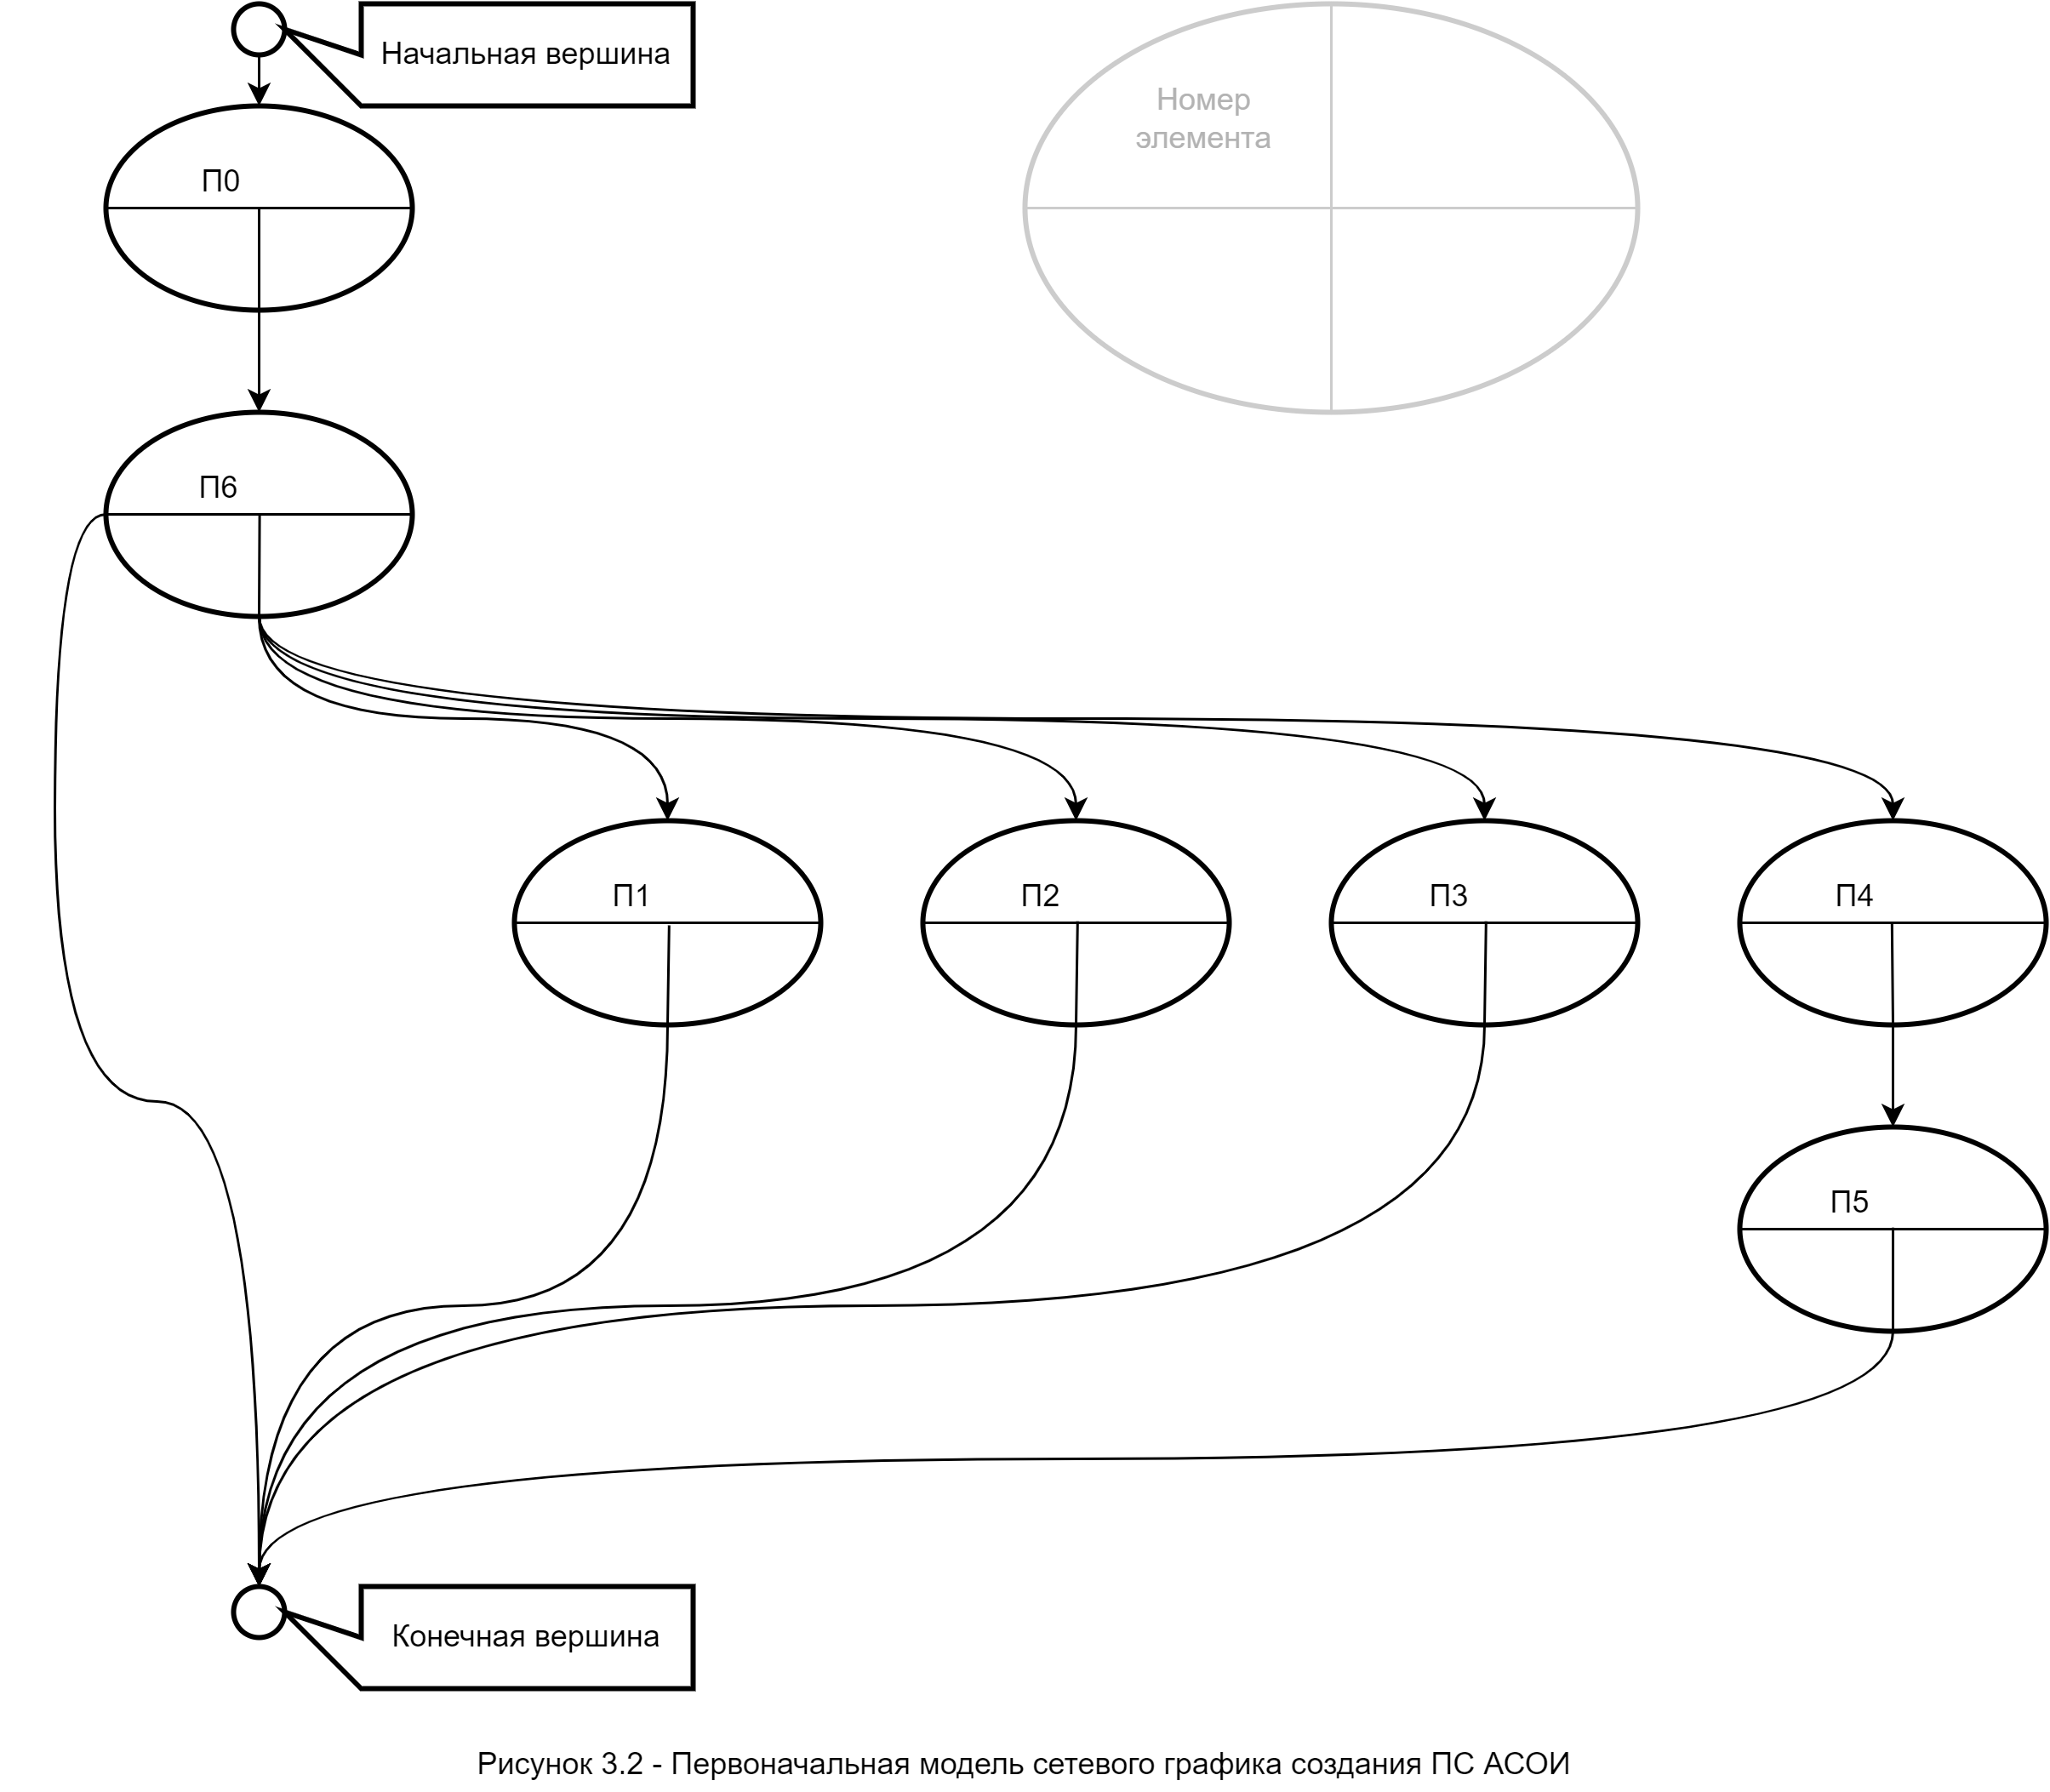
\includegraphics[width=16cm]
            {_docs/Рисунок3-2ПервоначальнаяМодельСетевогоГрафикаСозданияПСАСОИ.png}
        \caption{Первоначальная модель сетевого графика создания ПС АСОИ}
    \end{figure}

    \textbf{Сетевой график} - совокупность вершин и связей. Вершины графа имеют следующее назначение:
    \begin{enumerate}
        \item[1.] Начальная вершина - определяет начало создания ПС.
        \item[2.] Конечная вершина - определяет окончание создания ПС,
        если все связанные с этой вершиной приложения (промежуточные вершины) созданы.
        \item[3.] Промежуточная вершина - определяет разработку отдельного приложения (пользовательского или ЭП)
        или закупку системных и инструментальных программ.
    \end{enumerate}
   
    \textbf{Промежуточные вершины} делятся на три типа:
    \begin{enumerate}
        \item[1.] Вершина П0 - представляет набор системных и инструментальных программ,
        которые приобретаются и в процессе реализации не рассматривается.
        \item[2.] Вершина П6 - приложение эксплуатационного персонала,
        которое должно быть создано в первую очередь.
        \item[3.] Вершины П1 - П5 - пользовательские приложения,
        последовательность их создания определяется связями между этими приложениями.
    \end{enumerate}

    В каждой вершине представлена следующая информация:
    \begin{enumerate}
        \item[1.] Название приложения - П0, П1 и т.д.
        \item[2.] Стоимость вершины (экспертная оценка стоимости реализации приложения, представленного вершиной).
        Для П0 - стоимость системных и прикладных программ.
        Для остальных вершин - экспертная стоимость разработки соответствующего приложения.
    \end{enumerate}

    Связи между вершинами определяют рекомендуемую последовательность их реализации.

    \begin{figure}[ph!]
        \centering
        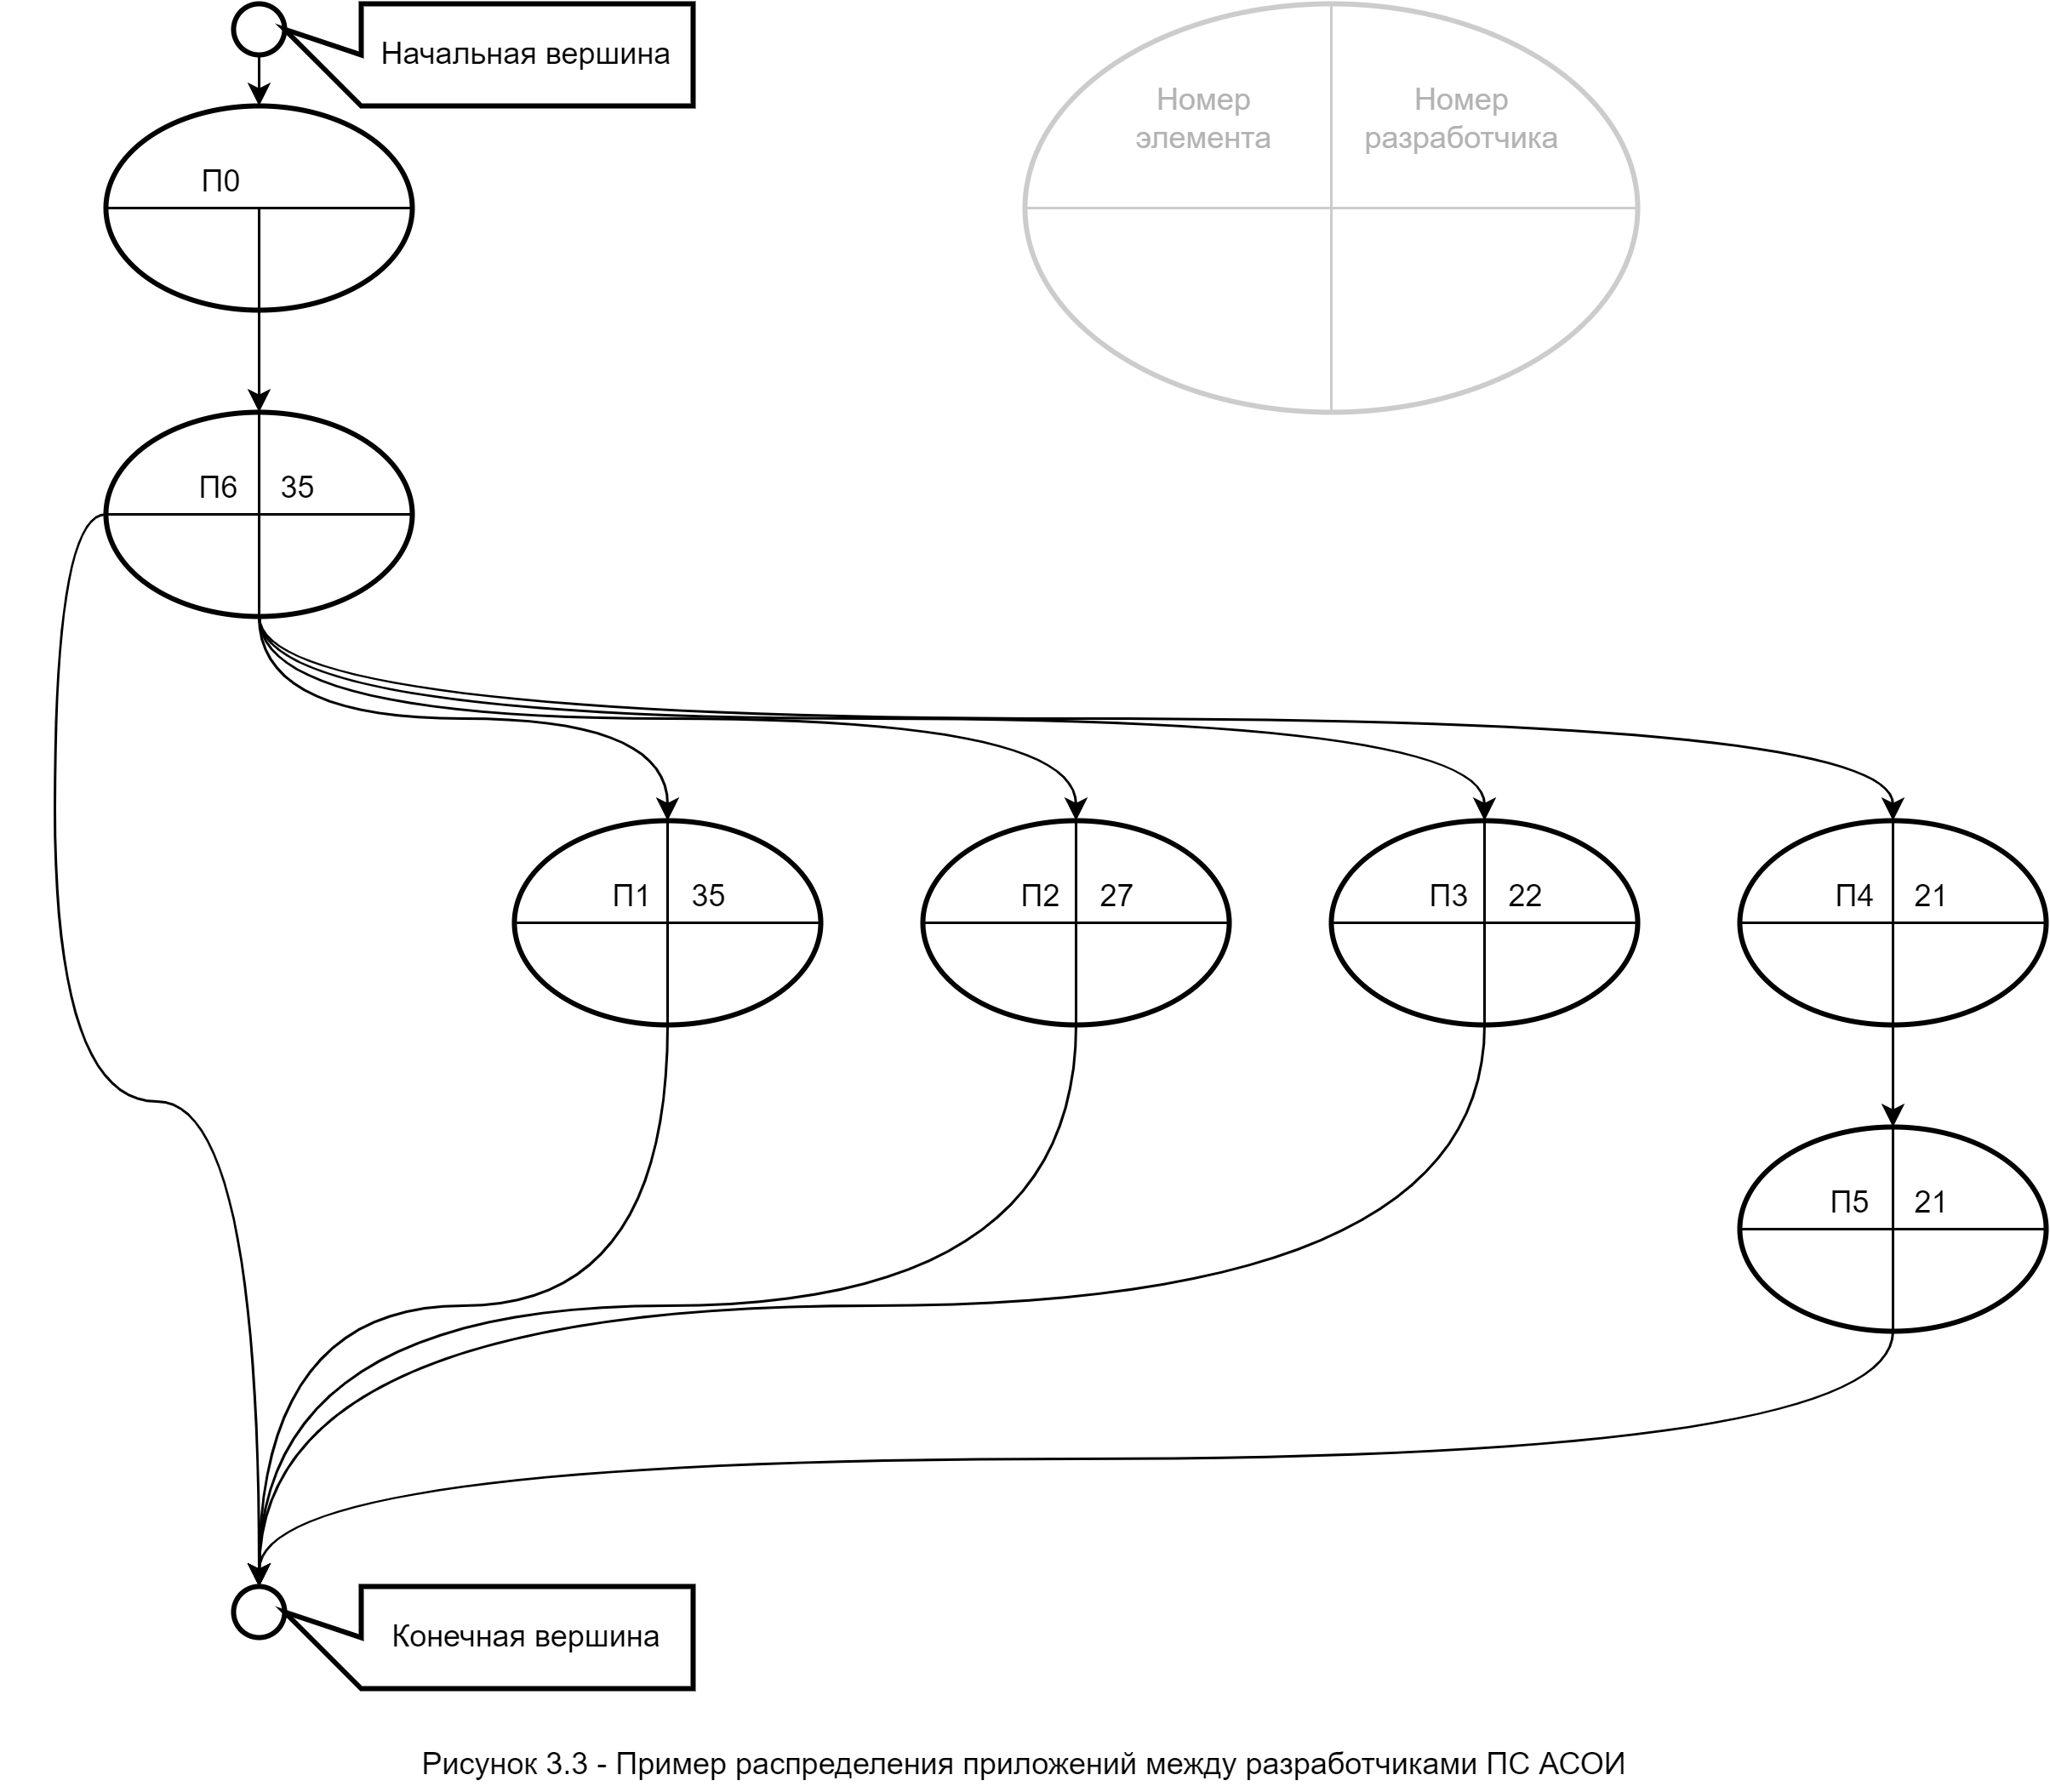
\includegraphics[width=16cm]
            {_docs/Рисунок3-3ПримерРаспределенияПриложенияМеждуРазработчикамиПСАСОИ.png}
        \caption{Первоначальная модель сетевого графика создания ПС АСОИ}
    \end{figure}

    \newpage
    \textbf{Распределение приложений между разработчиками} - это планирование реализации приложение заданным коллективом разработчиков. 
    
    Рассматривается два способа данной задачи:
    \begin{enumerate}
        \item[1.] С использованием методов оптимизации, рассмотренных в рамках дисциплины «Системный анализ и исследование операций» [3].
        Планирование включает построение оптимального плана реализации ПС коллективом разработчиков.
        В качестве критерия оптимизации можно использовать минимальное время или минимальная стоимость реализации ПС.
        Выполняется студентом самостоятельно для получения высокой оценки по КП!!!
        \item[2.] Путем «простого» подбора возможного варианта распределения приложений между разработчиками (оптимизация не применяется).
        Данный вариант рассматривается далее.
    \end{enumerate}

    Примечание. Создание П0 в планировании производства ПС не рассматривается, оно приобретается. Предполагается, что оно приобретено до начало реализации приложений ПС.
    
    Распределение разработчиков включает последовательность следующих действий:
    \begin{enumerate}
        \item[1.] Выбор списка разработчиков элементов АСОИ из табл. М.1 согласно заданному варианту АСОИ.
        % Список разработчиков следующий: 1, 2, 12, 15, 24 и 26.
        \item[2.] Выбор из заданного списка разработчиков, которые создают программы (см. табл. М.2, графа «Создание программ»).
        % В данном списке разработчиками программ являются 23, 24 и 25 разработчики.
    \end{enumerate}

    \begin{figure}[h!]
        \centering
        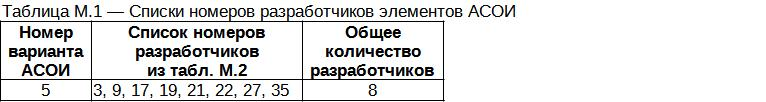
\includegraphics[]
            {_docs/ТаблицаМ1СпискиНомеровРазработчиковЭлементовАСОИ.jpg}
        \caption{Списки номеров разработчиков элементов АСОИ}
    \end{figure}

    \begin{figure}[h!]
        \centering
        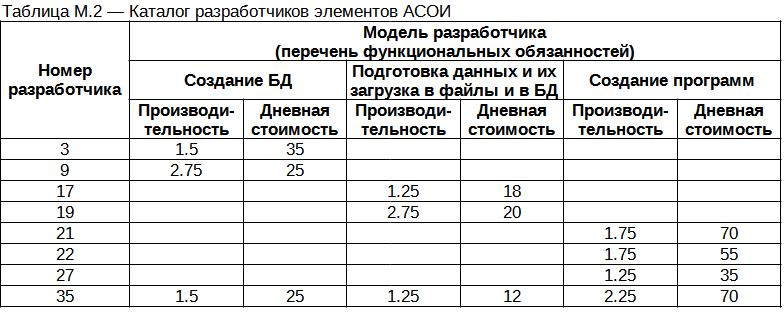
\includegraphics[width=16cm]
            {_docs/ТаблицаМ2КаталогРазработчиковЭлементовАСОИ.jpg}
        \caption{Каталог разработчиков элементов АСОИ}
    \end{figure}

    \begin{figure}[h!]
        \centering
        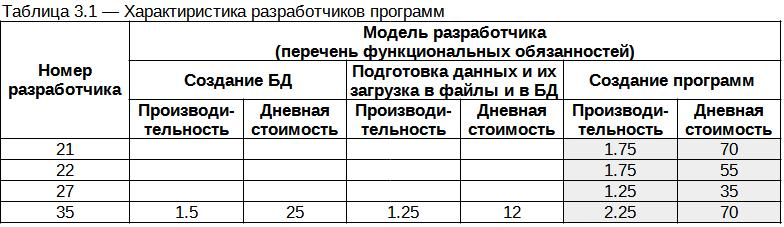
\includegraphics[width=16cm]
            {_docs/Таблица3-1ХарактеристикаРазработчиковПрограмм.jpg}
        \caption{Характеристика разработчиков программ}
    \end{figure}

    \newpage

    <<Номер разработчика>> раздал каждому П1, П2, П3, П4, П5, П6 по придуманому мной рисунку 3.5 (родная таблица М.2).

    <<Производительность>> взял из таблицы 3.1 (родная таблица М.2).

    <<Стоимость>> - ? Не даны данные!!! Пусть <<Стоимость>> = 36 из лабы 1.

    <<Трудоемкость реализации>> - ? Не даны данные!!! Пусть <<Трудоемкость реализации>> = 300.

    <<Время реализации>> = <<Трудоемкость реализации>> / <<Производительность>>

    \textbf{Для П1:} 300 / 2.25 = 133.33

    \textbf{Для П2:} 300 / 1.25 = 240.00

    \textbf{Для П3:} 300 / 1.75 = 171.43

    \textbf{Для П4:} 300 / 1.75 = 171.43

    \textbf{Для П5:} 300 / 1.75 = 171.43

    \textbf{Для П5:} 300 / 2.25 = 133.33

    <<Стоимость реализации>> = <<Время реализации>> * <<Дневная стоимость>>

    \textbf{Для П1:} 133.33 * 70.00 = 9 333.33

    \textbf{Для П2:} 240.00 * 35.00 = 8 400.00

    \textbf{Для П3:} 171.43 * 55.00 = 9 428.57

    \textbf{Для П4:} 171.43 * 70.00 = 12 000.00

    \textbf{Для П5:} 171.43 * 70.00 = 12 000.00

    \textbf{Для П6:} 133.33 * 70.00 = 9 333.33

    \begin{figure}[ph!]
        \centering
        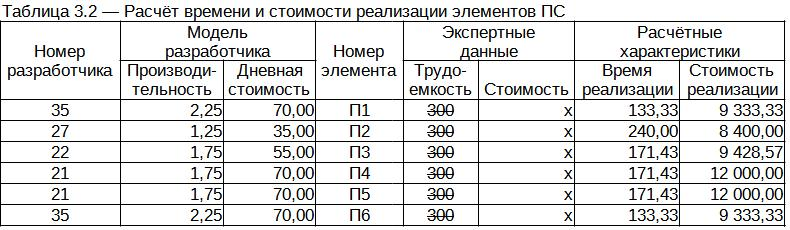
\includegraphics[width=16cm]
            {_docs/Таблица3-2РасчётВремениИСтоимостиРеализацииЭлементовПС.jpg}
        \caption{Расчёт времени и стоимости реализации элементов ПС}
    \end{figure}

    \begin{figure}[ph!]
        \centering
        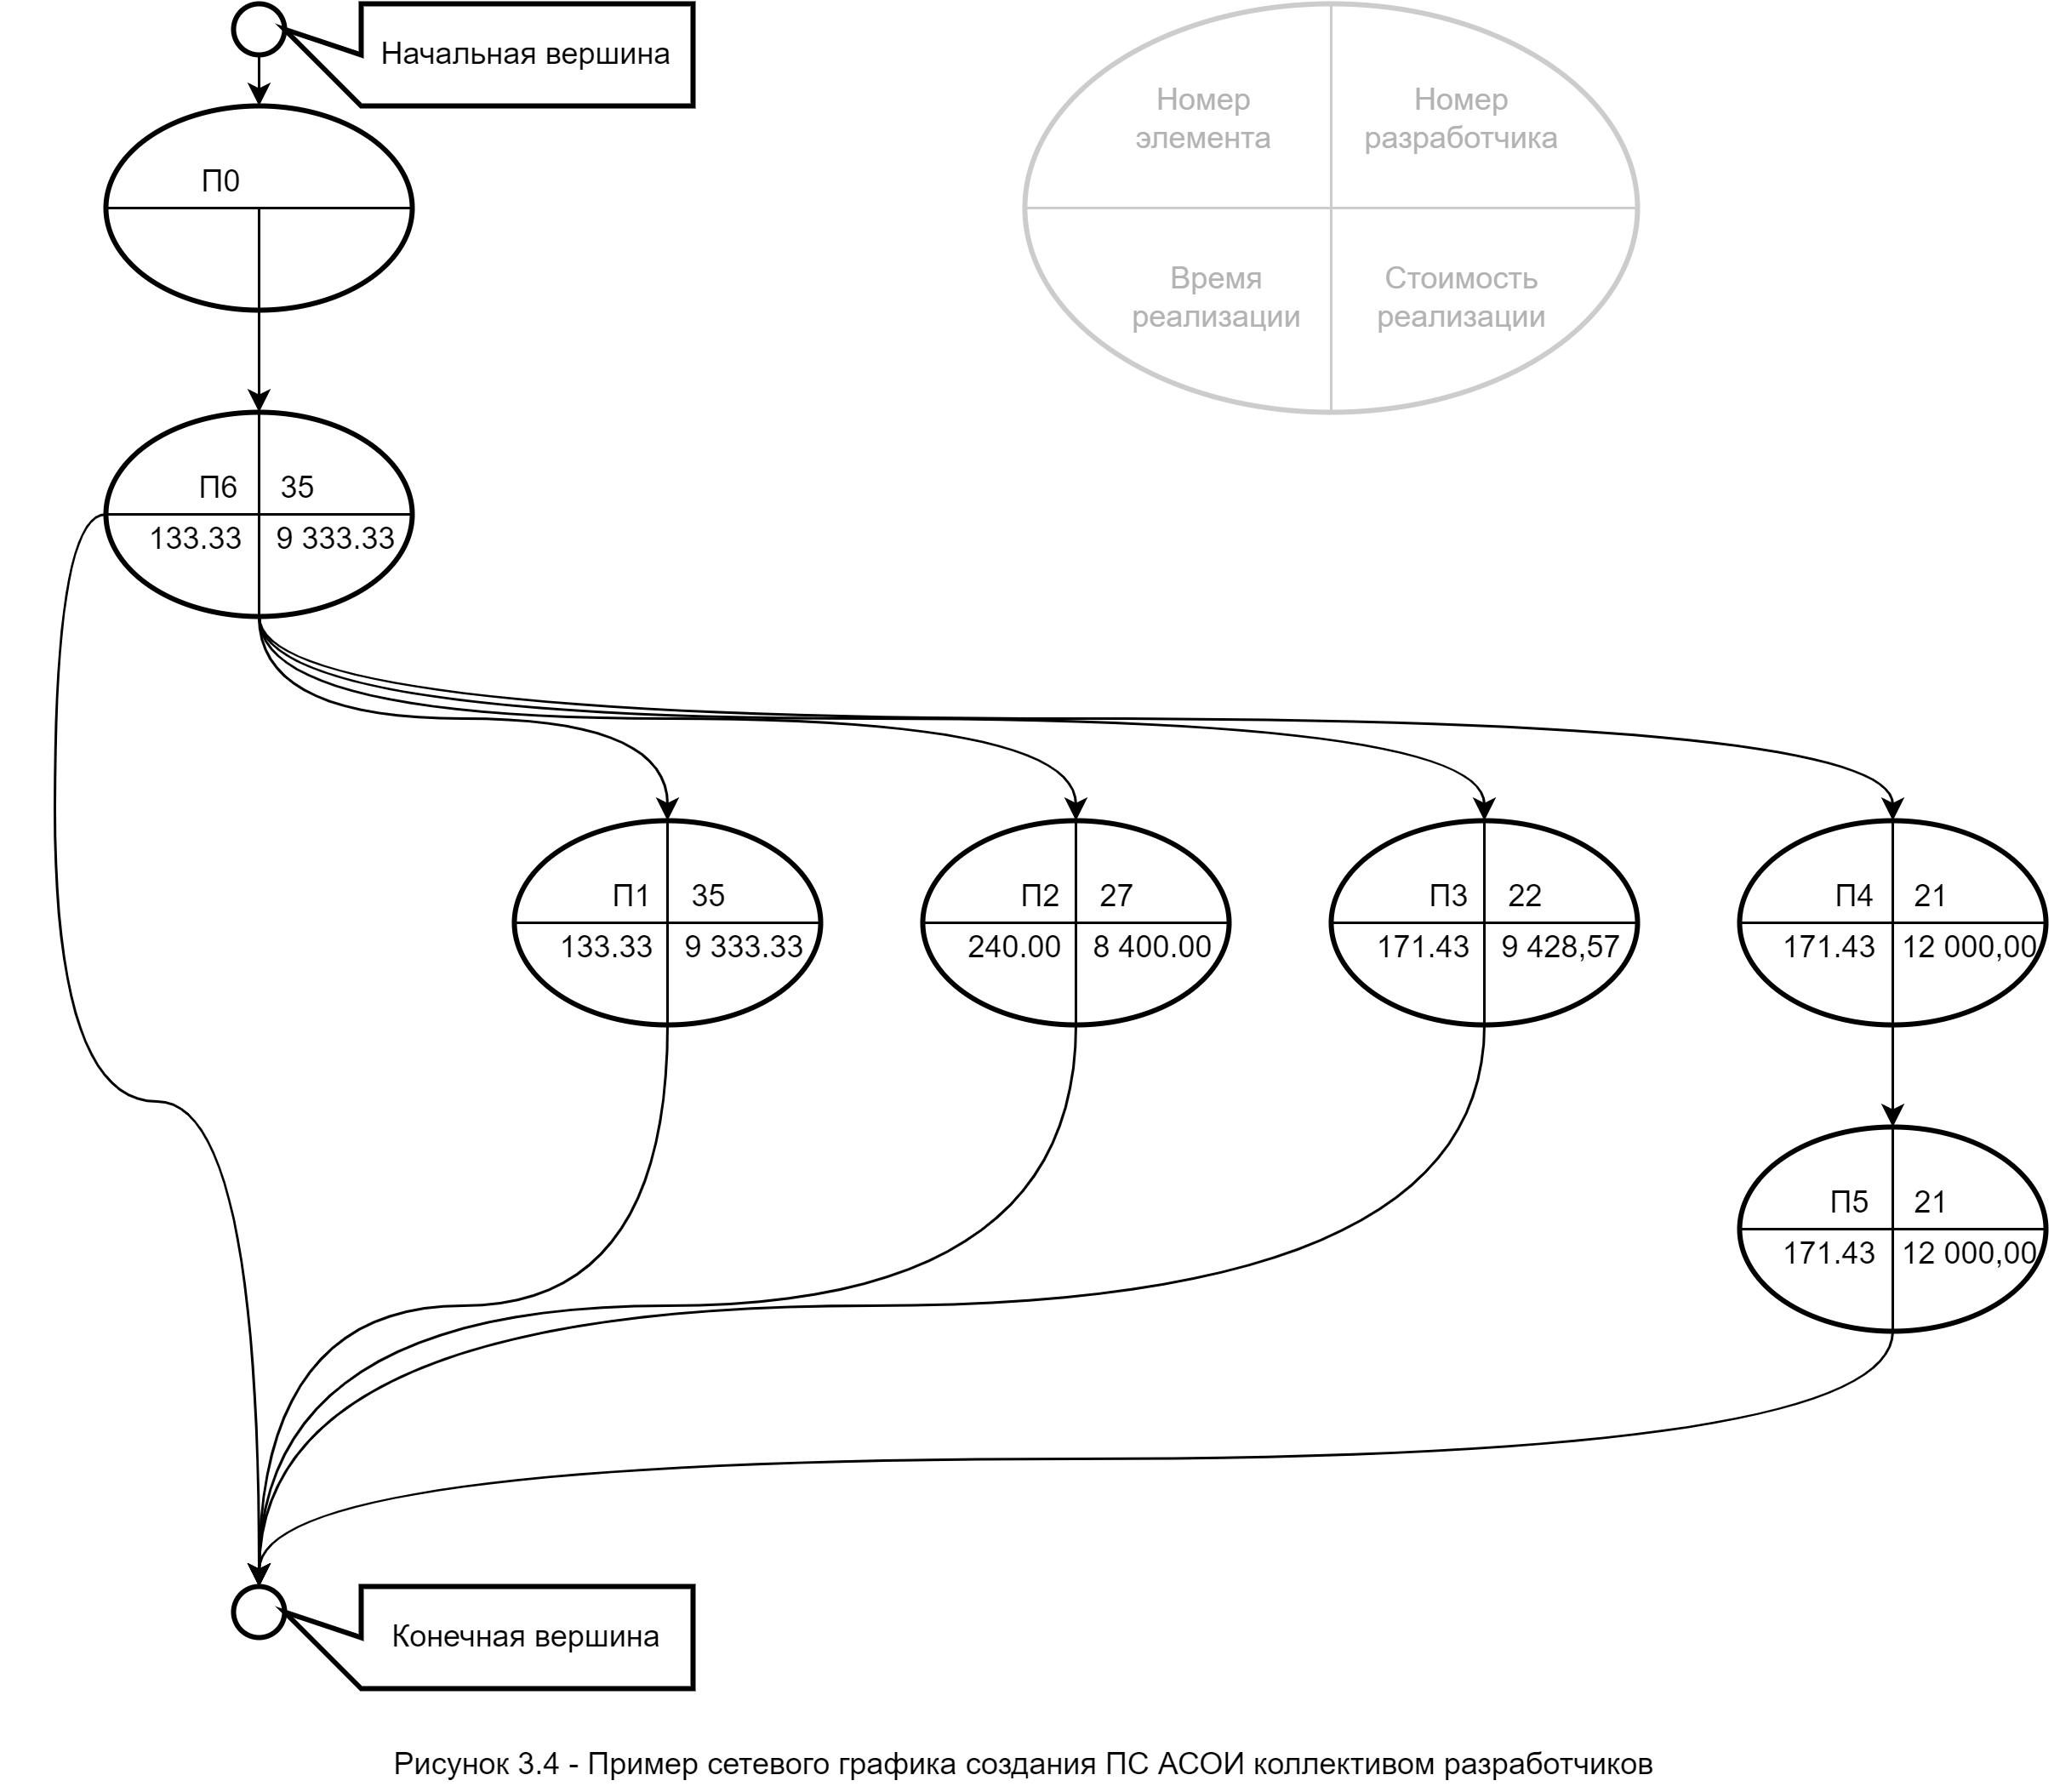
\includegraphics[width=16cm]
            {_docs/Рисунок3-4ПримерСетевогоГрафикаСозданияПСАСОИКоллективомРазработчиков.png}
        \caption{Пример сетевого графика создания ПС АСОИ коллективом разработчиков}
    \end{figure}

    \newpage
    \textbf{Пример разработки плана создания ПЭ АСОИ}.
    На основе сетевого графика разраба­тыва­ется план реализации приложений ПС заданным коллективом разработчиков. 

    \begin{figure}[ph!]
        \centering
        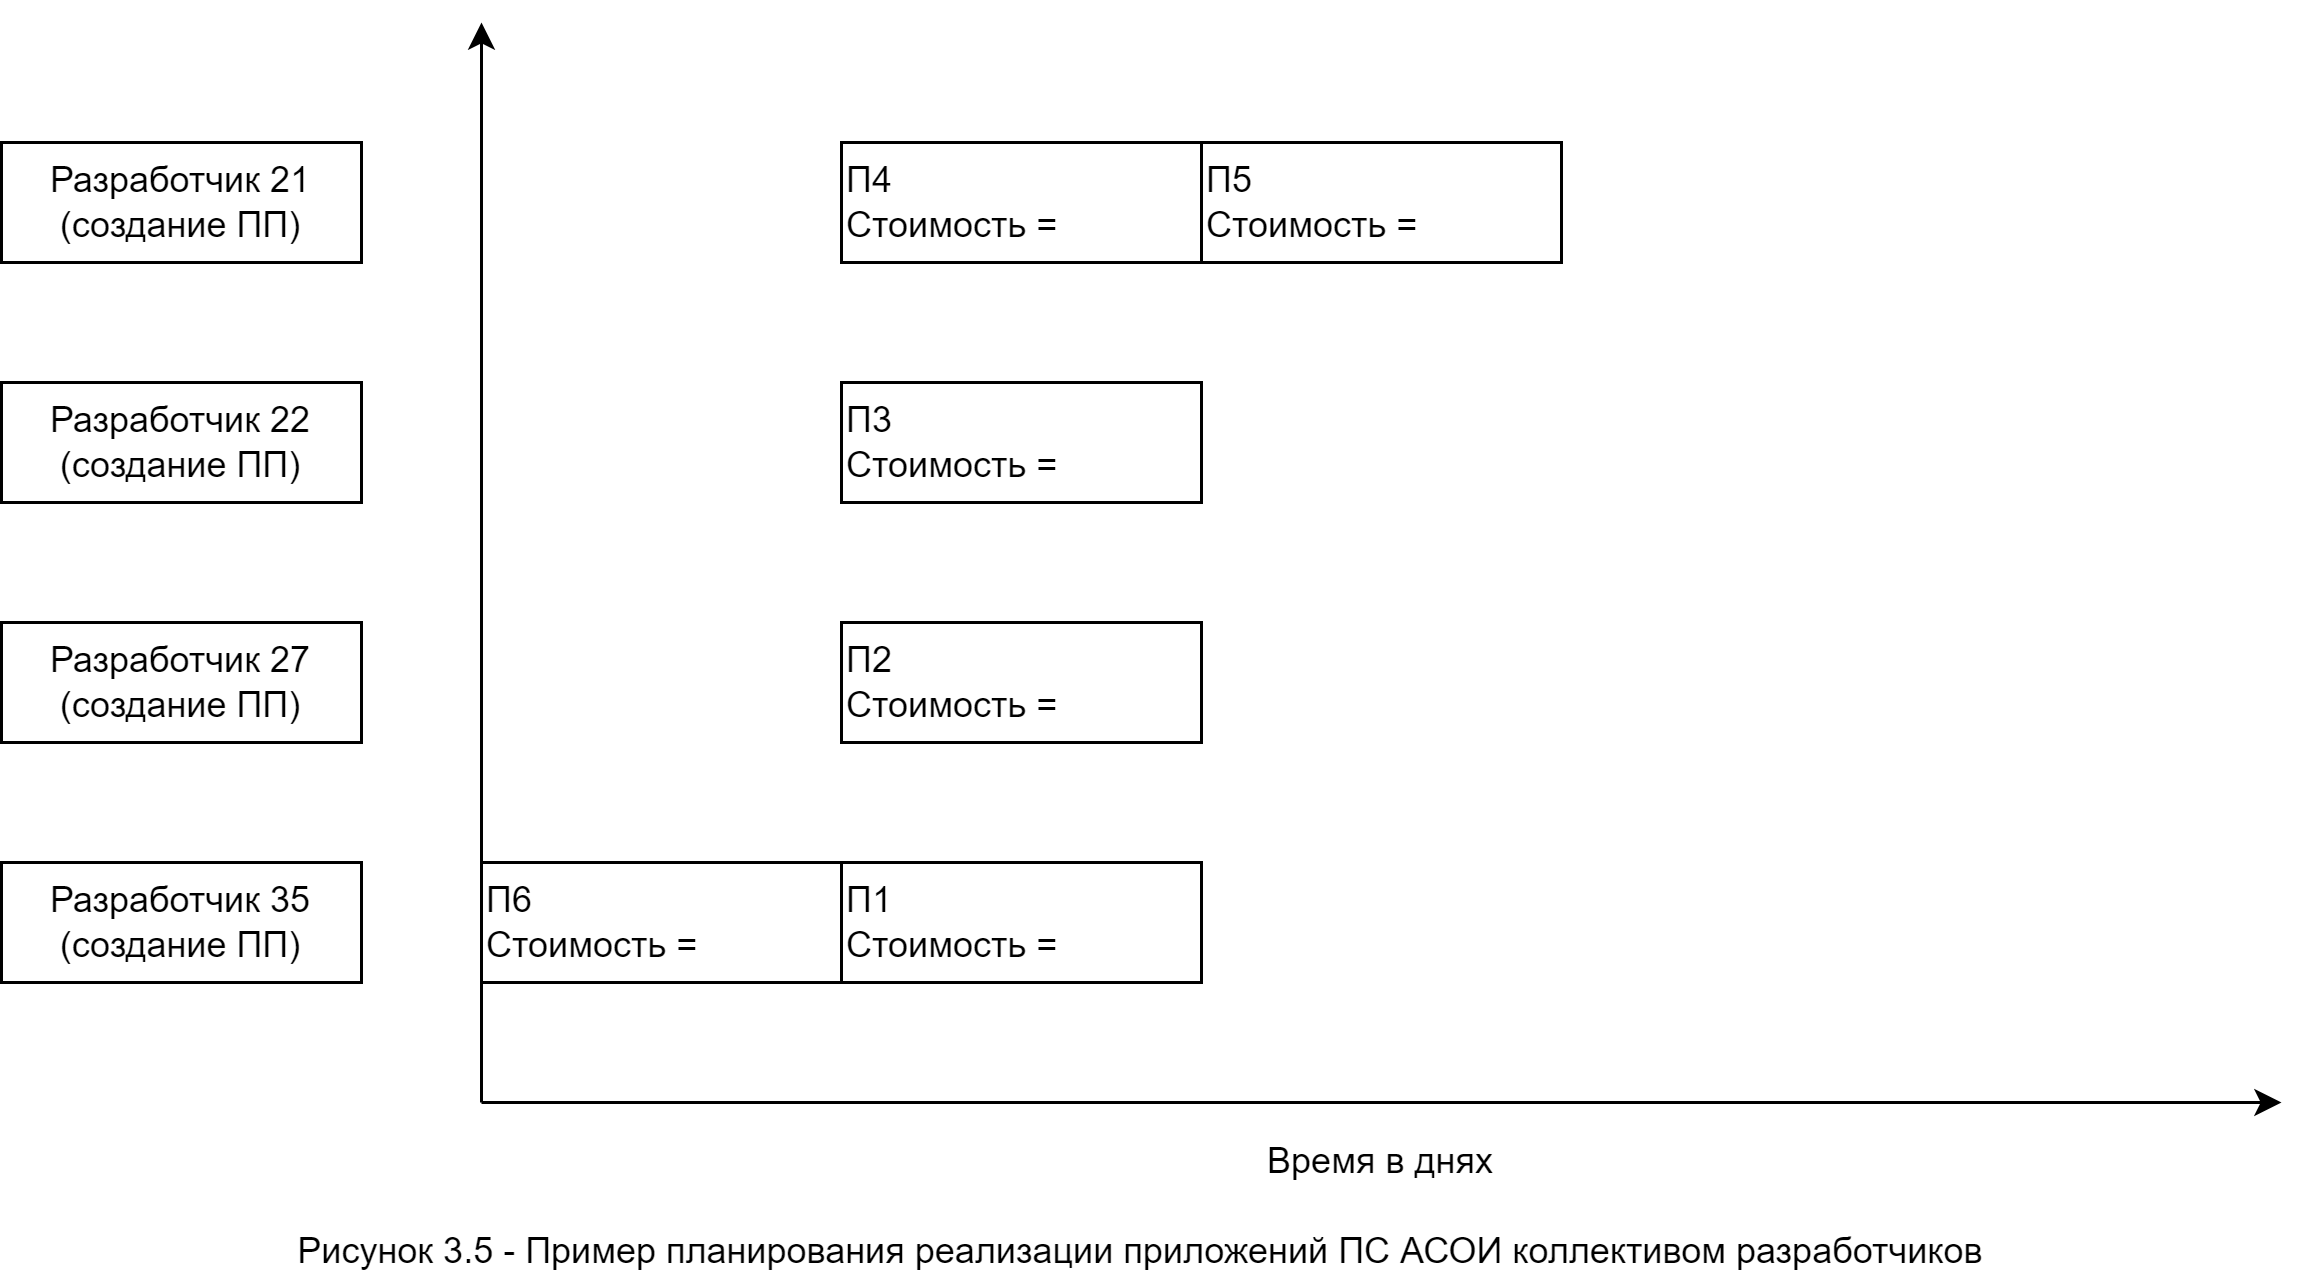
\includegraphics[width=16cm]
            {_docs/Рисунок3-5ПримерПланированияРеализацииПриложенийПСАСОИКоллективомРазработчиков.png}
        \caption{Пример планирования реализации приложений ПС АСОИ коллективом разработчиков}
    \end{figure}

    \paragraph{} \textbf{Пример деления ПС на очереди}

    На рисунке 4.1 приведен пример деления процесса создания ПС АСОИ на очереди.
    В качестве основы для деления ПС используется логическая структура ПС и оценки стоимости реализации отдельных элементов ПС.

    \begin{figure}[ph!]
        \centering
        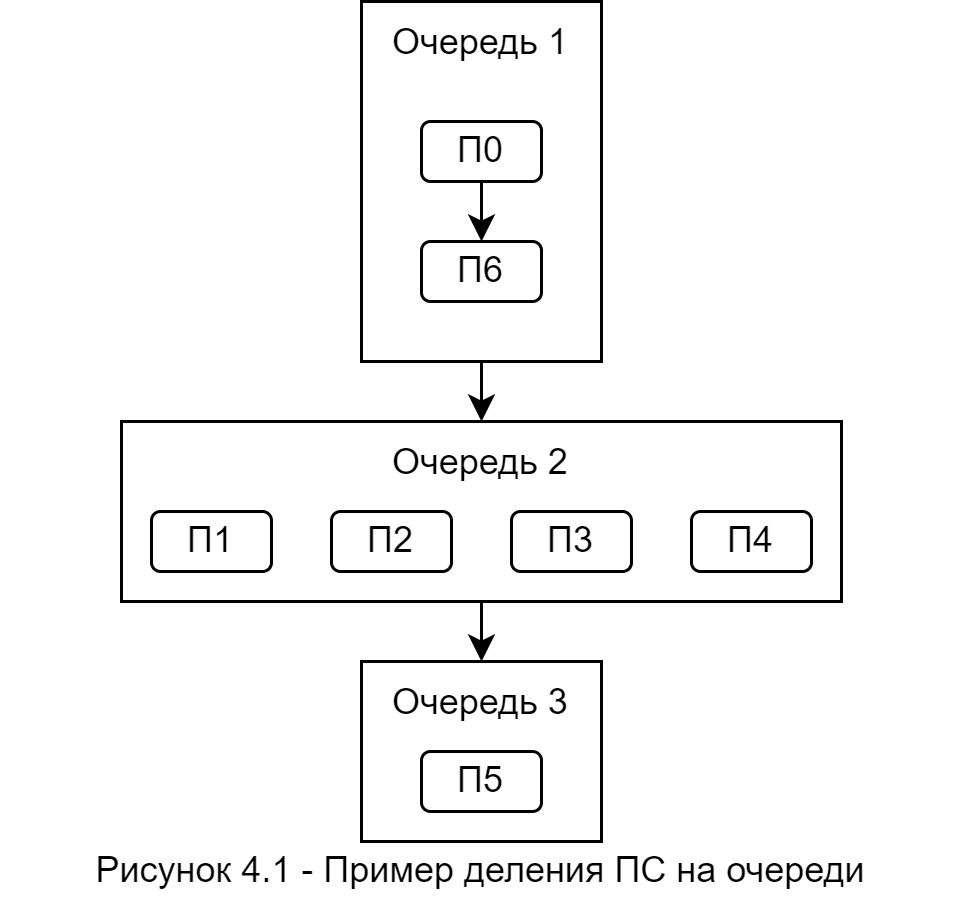
\includegraphics[]
            {_docs/Рисунок4-1ПримерДеленияПСНаОчереди.png}
        \caption{Пример деления ПС на очереди}
    \end{figure}
    
\end{document}
